\frame
{
\frametitle{Barnes-Hut Tree Code}
\framesubtitle{Idea}

\begin{center}
``Agrupar cuerpos cercanos y aproximarlos en un solo cuerpo''
\end{center}

\begin{itemize}
	\item Si el grupo está \blue{muy lejos}, se aproximan los efectos gravitacionales
		 utilizando el centro de masa.
	\item \green{Centro de masa}, promedio de las posiciones de un cuerpo en un grupo,
		 ponderado por la masa.
\end{itemize}
}

\frame
{
\frametitle{Barnes-Hut Tree Code}
\framesubtitle{Idea}

\green{Centro de Masa}

\begin{center}
Formalmente si \blue{dos cuerpos} con posiciones $(x_{1},y_{1})$, $(x_{2},y_{2})$ y
masas $m_{1}$, $m_{2}$, la masa total del centro de masa $(x,y)$ está dada por:
\end{center}

\begin{eqnarray}
	m &=& m_{1} + m_{2} \nonumber \\
	x &=& \frac{(x_{1}\cdot m_{1} + x_{2}\cdot m_{2})}{m} \nonumber \\
	y &=& \frac{(y_{1}\cdot m_{1} + y_{2}\cdot m_{2})}{m} \nonumber 
\end{eqnarray}

}

\frame
{
\frametitle{Barnes-Hut Tree Code}
\framesubtitle{Algoritmo}

\begin{itemize}
	\item Esquema inteligente para \blue{agrupar} cuerpos suficientemente cerca.
	\item Recursivamente \blue{divide} el conjunto de cuerpos en grupos
		guardándolos en un ``quad-tree''.
	\item Cada \blue{nodo} representa una región en un espacio de dos dimensiones.
	\item El nodo \blue{más alto} representa todo el espacio,
		y sus cuatro \blue{hijos} representan cuatro cuadrantes en el espacio,
\end{itemize}
}

\frame
{
\frametitle{Barnes-Hut Tree Code}
\framesubtitle{Aproximación}
\def\layersep{2.5cm}
\begin{center}
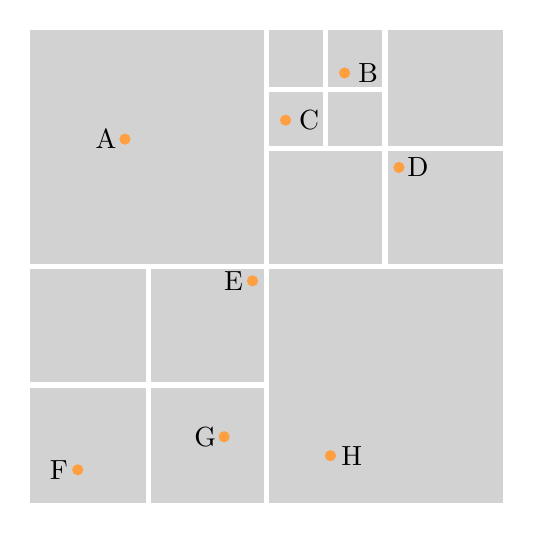
\begin{tikzpicture}[scale=0.6]

    \tikzstyle{square}=[rectangle,fill=gray!35, minimum size=6cm]
    \node[square] at (0,0) {};

    \draw[draw=white!50, line width=2pt] (-5,0)     -- (5,0)
                                         (0,5)      -- (0,-5)
                                         (2.5,5)    -- (2.5,0)
                                         (0,2.5)    -- (5,2.5)
                                         (0,3.75)   -- (2.5,3.75)
                                         (1.25,2.5) -- (1.25,5)
                                         (-2.5,0)   -- (-2.5,-5)
                                         (0,-2.5)   -- (-5,-2.5);


    \filldraw[draw=orange!75, fill=orange!75] (-3,2.7)    circle (3pt)
                                              (1.65,4.1)  circle (3pt)
                                              (0.4,3.1)   circle (3pt)
                                              (2.8,2.1)   circle (3pt)
                                              (-0.3,-0.3) circle (3pt)
                                              (-4,-4.3)   circle (3pt)
                                              (-0.9,-3.6) circle (3pt)
                                              (1.35,-4)   circle (3pt);

    \draw (-3.4,2.7)  node {A}
          (2.15,4.1)  node {B}
          (0.9,3.1)   node {C}
          (3.2,2.1)   node {D}
          (-0.7,-0.3) node {E}
          (-4.4,-4.3) node {F}
          (-1.3,-3.6) node {G}
          (1.8,-4)    node {H};

\end{tikzpicture}
\end{center}
}
	
\frame
{
\frametitle{Barnes-Hut Tree Code}
\framesubtitle{Aproximación}
\begin{itemize}
	\item Cada nodo \blue{externo}, representa un \red{único} cuerpo.
	\item Cada nodo \blue{interno}, representa el \red{grupo} de cuerpos debajo de ella,
			(guarda ``centro de masa'' y ``masa total'').
\end{itemize}
}


\frame
{
\frametitle{Barnes-Hut Tree Code}
\framesubtitle{Aproximación}

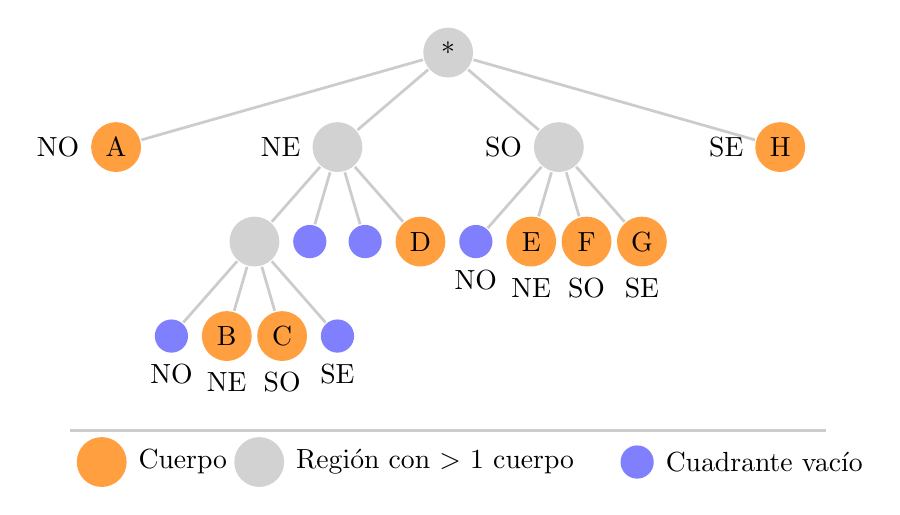
\begin{tikzpicture}[level 1/.style={sibling distance=10em},
                    level 2/.style={sibling distance=2.5em},
                    level distance = 1.5cm,
                    draw=gray!40,
                    fill=gray!40,
                    line width=1pt,
					scale=0.8]
    \tikzstyle{internal}=[circle,fill=gray!35,minimum size=18pt,inner sep=2pt]
    \tikzstyle{external}=[internal, fill=orange!75];
    \tikzstyle{empty}=[internal, fill=blue!50, minimum size=12pt];

    \node[internal] {*}
        child { node[external,label=left:NO] {A}}
        child { node[internal,label=left:NE] {}
            child { node[internal] {}
                child { node[empty,label=below:NO] {} }
                child { node[external,label=below:NE] {B} }
                child { node[external,label=below:SO] {C} }
                child { node[empty,label=below:SE] {} }
            }
            child { node[empty] {} }
            child { node[empty] {} }
            child { node[external] {D} }
        }
        child { node[internal,label=left:SO] {}
            child { node[empty,label=below:NO] {}}
            child { node[external,label=below:NE] {E}}
            child { node[external,label=below:SO] {F}}
            child { node[external,label=below:SE] {G}}
        }
        child { node[external,label=left:SE] {H}};

        \draw (-6,-6) -- (6,-6);
        \node[external, label=right:Cuerpo] at (-5.5,-6.5) {};
        \node[internal,label=right:Región con $>$ 1 cuerpo] at (-3,-6.5) {};
        \node[empty,label=right:Cuadrante vacío] at (3,-6.5){};

\end{tikzpicture}
}

\frame
{
\frametitle{Barnes-Hut Tree Code}
\framesubtitle{Cálculo de la fuerza}

\begin{itemize}
	\item En un \blue{cuerpo} particular.
	 \begin{itemize}
	 	\item Recorrer los nodos del árbol, partiendo de la raíz.
	 \end{itemize}
	\item Centro de masa de un \blue{nodo interno}:
	\begin{itemize}
		\item \green{Si} lo suficientemente lejos del cuerpo.
		\begin{itemize}
			\item Se aproximan los cuerpos contenidos. (con centro de masa y masa total)
		\end{itemize}
		\item \red{No} lo suficientemente lejos del cuerpo.
		\begin{itemize}
			\item Recorrer los sub-árboles recursivamente.
		\end{itemize}
	\end{itemize}
\end{itemize}
}

\frame
{
\frametitle{Barnes-Hut Tree Code}
\framesubtitle{Cálculo de la fuerza}

\begin{itemize}
	\item ¿Cómo determinarlo?
	\begin{itemize}
		\item $ Cociente\ =\ \frac{\text{ancho región nodo }(s)}{\text{distancia Cuerpo-CM }(d)}$
	\end{itemize}
	\item Después, comparar con un valor umbral $\theta$.
	\begin{itemize}
		\item Si \blue{$\frac{s}{d} < \theta$}, entonces el nodo interno esta lo suficiente \blue{lejos}.
		\item Ajustando \blue{$\theta$}, podemos cambiar la \green{velocidad} y la \green{precisión} de la simulación.
		\item Se suele utilizar \blue{$\theta = 0.5$}. Si \red{$\theta = 0$}, degenera (fuerza bruta).
	\end{itemize}
\end{itemize}
}

\frame
{
\frametitle{Barnes-Hut Tree Code}
\framesubtitle{Construyendo un árbol}

Si queremos ingresar el \blue{cuerpo b} en el árbol con raíz en el \red{nodo x}.

\begin{enumerate}
	\item<1-> Si el \red{nodo x} no contiene un cuerpo, poner el nuevo \blue{cuerpo b} ahí.
	\item<2-> Si el \red{nodo x} es un nodo \green{interno}, actualizar el CM
		y M. (Recursivamente inserta el \blue{cuerpo b} en el cuadrante apropiado).
	\item<3-> Si el \red{nodo x} es un nodo \green{externo}, digamos que contiene un \blue{cuerpo
		   c}, entonces hay \red{dos} cuerpos, \blue{b} y \blue{c} en la misma región.
		\begin{itemize}
			\item<4-> \blue{Subdivide} la región creando cuatro hijos.
			\item<5-> Entonces, recursivamente \blue{inserta ambos} cuerpos, b y c, en el cuadrante apropiado.
			\item<6-> \blue{Recursividad!}
				%Puesto que b y c todavía pueden terminar en el mismo cuadrantes, podrian
				% haber varias subdivisiones durante una inserción simple.
			\item<7-> Finalmente, actualizar el CM y M de \red{x}.
		\end{itemize}
\end{enumerate}
}

\frame
{
\frametitle{Barnes-Hut Tree Code}
\framesubtitle{Construyendo un árbol}

\begin{itemize}
	\item Ejemplo, 5 cuerpos.
	\begin{itemize}
		\item Convención ramas, de izquierda a derecha (NO, NE, SO y SE).
	\end{itemize}
\end{itemize}

\begin{center}
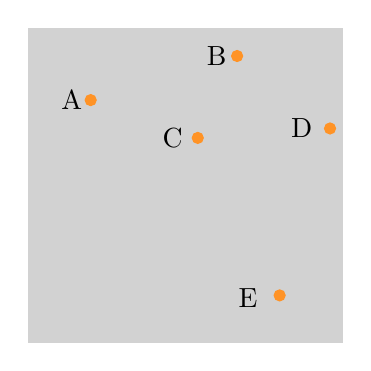
\begin{tikzpicture}[scale=0.4]
    \tikzstyle{square}=[rectangle,fill=gray!35, minimum size=4cm]
    \node[square] at (0,0) {};
    \filldraw[draw=orange!85, fill=orange!85] (-3,2.7)    circle (5pt)
                                              (1.65,4.1)  circle (5pt)
                                              (0.4,1.5)   circle (5pt)
                                              (4.6,1.8)   circle (5pt)
                                              (3,-3.5)    circle (5pt);
    \draw (-3.6,2.7)  node {A}
          (1,4.1)  node {B}
          (-0.4,1.5)   node {C}
          (3.7,1.8)   node {D}
          (2,-3.6) node {E};
\end{tikzpicture}
\hspace{0.5cm}
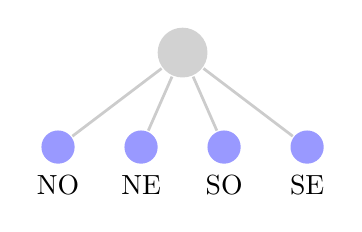
\begin{tikzpicture}[level 1/.style={sibling distance=5em, level distance=2cm},
                    level distance = 2cm,
                    draw=gray!40,
                    fill=gray!40,
                    line width=1pt,
                    scale=0.6]
    \tikzstyle{internal}=[circle,fill=gray!35,minimum size=18pt,inner sep=2pt]
    \tikzstyle{external}=[internal, fill=orange!85];
    \tikzstyle{externaldisable}=[external, fill=orange!35];
    \tikzstyle{empty}=[internal, fill=blue!40, minimum size=12pt];
    \tikzstyle{actual}=[internal, draw=blue!50, minimum size=12pt,line width=2pt];

    \node[internal] {}
        child { node[empty,label=below:NO] {}}
        child { node[empty,label=below:NE] {} }
        child { node[empty,label=below:SO] {} }
        child { node[empty,label=below:SE] {} };
\end{tikzpicture}
\end{center}

}

\frame
{
\frametitle{Barnes-Hut Tree Code}
\framesubtitle{Construyendo un árbol}

\begin{itemize}
    \item Agregar cuerpo A.
    \begin{itemize}
        \item Encaja en el cuadrante NO de la raíz.
    \end{itemize}
\end{itemize}
\begin{center}
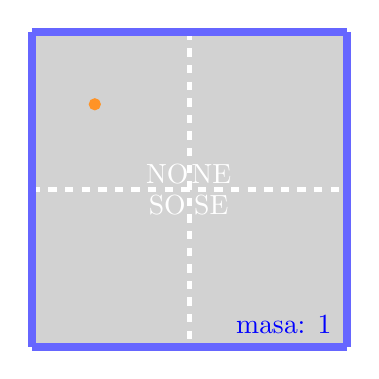
\begin{tikzpicture}[scale=0.4]
    \tikzstyle{square}=[rectangle,fill=gray!35, minimum size=4cm]
    \node[square] at (0,0) {};
    \draw[draw=white!50, line width=2pt,dashed] (-5,0)     -- (5,0)
                                         (0,5)      -- (0,-5);
    \draw[draw=blue!60, line width=3pt] (-5,5) -- (5,5)
                                        (5,5)  -- (5,-5)
                                        (5,-5) -- (-5,-5)
                                        (-5,-5)-- (-5,5);

    \filldraw[draw=orange!85, fill=orange!85] (-3,2.7)    circle (5pt);


    \draw[blue] (3,-4.3)  node {masa: 1};
    \draw[white] (-0.7,0.5) node {NO};
    \draw[white] (-0.7,-0.5) node {SO};
    \draw[white] (0.7,0.5) node {NE};
    \draw[white] (0.7,-0.5) node {SE};

\end{tikzpicture}
\hspace{0.5cm}
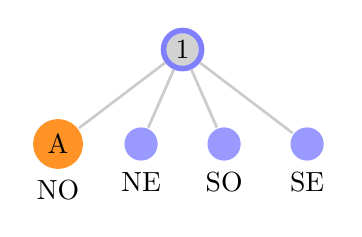
\begin{tikzpicture}[level 1/.style={sibling distance=5em, level distance=2cm},
                    level distance = 2cm,
                    draw=gray!40,
                    fill=gray!40,
                    line width=1pt,
                    scale=0.6]
    \tikzstyle{internal}=[circle,fill=gray!35,minimum size=18pt,inner sep=2pt]
    \tikzstyle{external}=[internal, fill=orange!85];
    \tikzstyle{externaldisable}=[external, fill=orange!35];
    \tikzstyle{empty}=[internal, fill=blue!40, minimum size=12pt];
    \tikzstyle{actual}=[internal, draw=blue!50, minimum size=12pt,line width=2pt];


    \node[actual] {1}
        child { node[external,label=below:NO] {A}}
        child { node[empty,label=below:NE] {} }
        child { node[empty,label=below:SO] {} }
        child { node[empty,label=below:SE] {} };
\end{tikzpicture}

\end{center}
}

\frame
{
\frametitle{Barnes-Hut Tree Code}
\framesubtitle{Construyendo un árbol}

\begin{itemize}
    \item Agregar cuerpo B.
    \begin{itemize}
        \item Encaja en el cuadrante NE de la raíz.
    \end{itemize}
\end{itemize}
\begin{center}
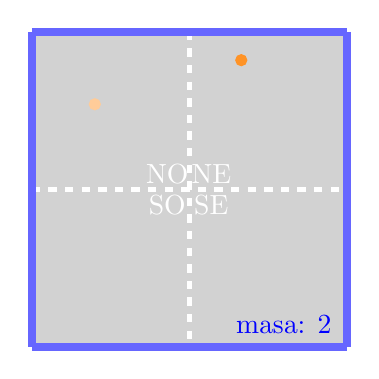
\begin{tikzpicture}[scale=0.4]
    \tikzstyle{square}=[rectangle,fill=gray!35, minimum size=4cm]
    \node[square] at (0,0) {};
    \draw[draw=white!50, line width=2pt,dashed] (-5,0)     -- (5,0)
                                         (0,5)      -- (0,-5);
    \draw[draw=blue!60, line width=3pt] (-5,5) -- (5,5)
                                        (5,5)  -- (5,-5)
                                        (5,-5) -- (-5,-5)
                                        (-5,-5)-- (-5,5);

    \filldraw[draw=orange!40, fill=orange!40] (-3,2.7)    circle (5pt);

    \filldraw[draw=orange!85, fill=orange!85] (1.65,4.1)  circle (5pt);

    \draw[blue] (3,-4.3)  node {masa: 2};
    \draw[white] (-0.7,0.5) node {NO};
    \draw[white] (-0.7,-0.5) node {SO};
    \draw[white] (0.7,0.5) node {NE};
    \draw[white] (0.7,-0.5) node {SE};

\end{tikzpicture}
\hspace{0.5cm}
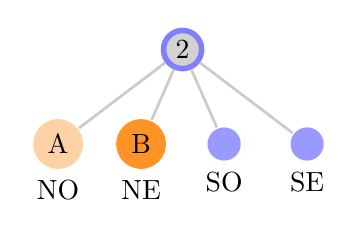
\begin{tikzpicture}[level 1/.style={sibling distance=5em, level distance=2cm},
                    level distance = 2cm,
                    draw=gray!40,
                    fill=gray!40,
                    line width=1pt,
                    scale=0.6]
    \tikzstyle{internal}=[circle,fill=gray!35,minimum size=18pt,inner sep=2pt]
    \tikzstyle{external}=[internal, fill=orange!85];
    \tikzstyle{externaldisable}=[external, fill=orange!35];
    \tikzstyle{empty}=[internal, fill=blue!40, minimum size=12pt];
    \tikzstyle{actual}=[internal, draw=blue!50, minimum size=12pt,line width=2pt];


    \node[actual] {2}
        child { node[externaldisable,label=below:NO] {A}}
        child { node[external,label=below:NE] {B} }
        child { node[empty,label=below:SO] {} }
        child { node[empty,label=below:SE] {} };
\end{tikzpicture}

\end{center}
}

\frame
{
\frametitle{Barnes-Hut Tree Code}
\framesubtitle{Construyendo un árbol}

\begin{itemize}
    \item Agregar cuerpo C.
    \begin{itemize}
        \item Cuadrante NE ocupado por B, se crea rama y se insertan los dos.
    \end{itemize}
\end{itemize}
\begin{center}
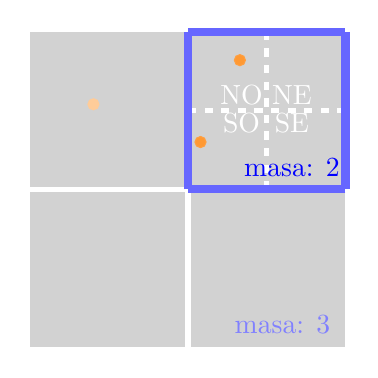
\begin{tikzpicture}[scale=0.4]
    \tikzstyle{square}=[rectangle,fill=gray!35, minimum size=4cm]
    \node[square] at (0,0) {};
    \draw[draw=white!30, line width=2pt] (-5,0)     -- (5,0)
                                         (0,5)      -- (0,-5);

    \draw[draw=white!30, line width=2pt, dashed] (2.5,5)    -- (2.5,0)
                                                 (0,2.5)    -- (5,2.5);
    \draw[draw=blue!60, line width=3pt] (0,5) -- (5,5)
                                        (5,5)  -- (5,0)
                                        (5,0) -- (0,0)
                                        (0,0)-- (0,5);

    \filldraw[draw=orange!40, fill=orange!40] (-3,2.7)    circle (5pt);

    \filldraw[draw=orange!75, fill=orange!80] (1.65,4.1)  circle (5pt)
                                              (0.4,1.5)   circle (5pt);

    \draw[blue] (3.3,0.7)  node {masa: 2};
    \draw[blue!50] (3,-4.3)  node {masa: 3};
    \draw[white] (1.7,3) node {NO};
    \draw[white] (1.7,2.1) node {SO};
    \draw[white] (3.3,3) node {NE};
    \draw[white] (3.3,2.1) node {SE};

\end{tikzpicture}
\hspace{0.5cm}
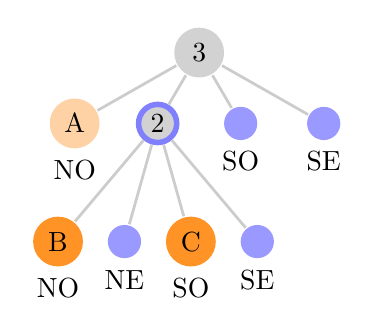
\begin{tikzpicture}[level 1/.style={sibling distance=5em, level distance=1.5cm},
                    level 2/.style={sibling distance=4em,level distance=2.5cm},
                    level distance = 2cm,
                    draw=gray!40,
                    fill=gray!40,
                    line width=1pt,
                    scale=0.6]
    \tikzstyle{internal}=[circle,fill=gray!35,minimum size=18pt,inner sep=2pt]
    \tikzstyle{external}=[internal, fill=orange!85];
    \tikzstyle{externaldisable}=[external, fill=orange!35];
    \tikzstyle{empty}=[internal, fill=blue!40, minimum size=12pt];
    \tikzstyle{actual}=[internal, draw=blue!50, minimum size=12pt,line width=2pt];


    \node[internal] {3}
        child { node[externaldisable,label=below:NO] {A}}
        child { node[actual] {2}
                child { node[external,label=below:NO] {B} }
                child { node[empty,label=below:NE] {} }
                child { node[external,label=below:SO] {C} }
                child { node[empty,label=below:SE] {} }
            }
        child { node[empty,label=below:SO] {} }
        child { node[empty,label=below:SE] {} };
\end{tikzpicture}
\end{center}
}

\frame
{
\frametitle{Barnes-Hut Tree Code}
\framesubtitle{Construyendo un árbol}

\begin{itemize}
    \item Agregar cuerpo D.
    \begin{itemize}
        \item Encaja en el cuadrante SE de la rama.
    \end{itemize}
\end{itemize}
\begin{center}
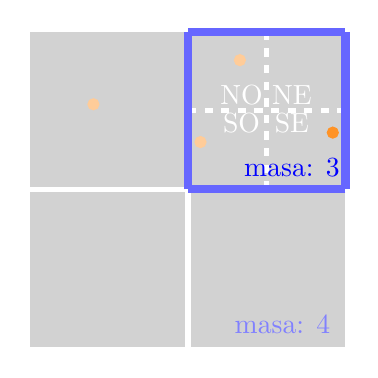
\begin{tikzpicture}[scale=0.4]
    \tikzstyle{square}=[rectangle,fill=gray!35, minimum size=4cm]
    \node[square] at (0,0) {};
    \draw[draw=white!30, line width=2pt] (-5,0)     -- (5,0)
                                         (0,5)      -- (0,-5);

    \draw[draw=white!30, line width=2pt, dashed] (2.5,5)    -- (2.5,0)
                                                 (0,2.5)    -- (5,2.5);
    \draw[draw=blue!60, line width=3pt] (0,5) -- (5,5)
                                        (5,5)  -- (5,0)
                                        (5,0) -- (0,0)
                                        (0,0)-- (0,5);

    \filldraw[draw=orange!40, fill=orange!40] (-3,2.7)    circle (5pt)
                                              (1.65,4.1)  circle (5pt)
                                              (0.4,1.5)   circle (5pt);

    \filldraw[draw=orange!85, fill=orange!85] (4.6,1.8)   circle (5pt);

    \draw[blue] (3.3,0.7)  node {masa: 3};
    \draw[blue!50] (3,-4.3)  node {masa: 4};
    \draw[white] (1.7,3) node {NO};
    \draw[white] (1.7,2.1) node {SO};
    \draw[white] (3.3,3) node {NE};
    \draw[white] (3.3,2.1) node {SE};

\end{tikzpicture}
\hspace{0.5cm}
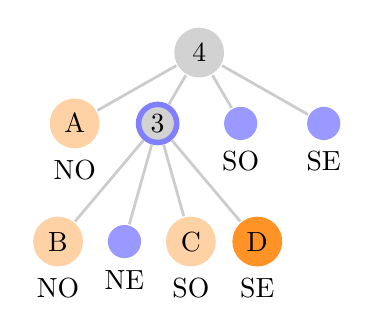
\begin{tikzpicture}[level 1/.style={sibling distance=5em, level distance=1.5cm},
                    level 2/.style={sibling distance=4em,level distance=2.5cm},
                    level distance = 1.5cm,
                    draw=gray!40,
                    fill=gray!40,
                    line width=1pt,
                    scale=0.6]
    \tikzstyle{internal}=[circle,fill=gray!35,minimum size=18pt,inner sep=2pt]
    \tikzstyle{external}=[internal, fill=orange!85];
    \tikzstyle{externaldisable}=[external, fill=orange!35];
    \tikzstyle{empty}=[internal, fill=blue!40, minimum size=12pt];
    \tikzstyle{actual}=[internal, draw=blue!50, minimum size=12pt,line width=2pt];


    \node[internal] {4}
        child { node[externaldisable,label=below:NO] {A}}
        child { node[actual] {3}
                child { node[externaldisable,label=below:NO] {B} }
                child { node[empty,label=below:NE] {} }
                child { node[externaldisable,label=below:SO] {C} }
                child { node[external,label=below:SE] {D} }
        }
        child { node[empty,label=below:SO] {} }
        child { node[empty,label=below:SE] {} };
\end{tikzpicture}
\end{center}
}

\frame
{
\frametitle{Barnes-Hut Tree Code}
\framesubtitle{Construyendo un árbol}

\begin{itemize}
	\item Agregar cuerpo E.
	\begin{itemize}
		\item Encaja en el cuadrante SE de la raíz.
	\end{itemize}
\end{itemize}
\begin{center}
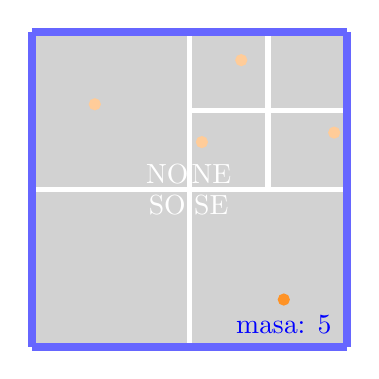
\begin{tikzpicture}[scale=0.4]

    \tikzstyle{square}=[rectangle,fill=gray!35, minimum size=4cm]
    \node[square] at (0,0) {};
    \draw[draw=white!50, line width=2pt] (-5,0)     -- (5,0)
                                         (0,5)      -- (0,-5)
                                         (2.5,5)    -- (2.5,0)
                                         (0,2.5)    -- (5,2.5);
    \draw[draw=blue!60, line width=3pt] (-5,5) -- (5,5)
                                        (5,5)  -- (5,-5)
                                        (5,-5) -- (-5,-5)
                                        (-5,-5)-- (-5,5);

    \filldraw[draw=orange!40, fill=orange!40] (-3,2.7)    circle (5pt)
                                              (1.65,4.1)  circle (5pt)
                                              (0.4,1.5)   circle (5pt)
                                              (4.6,1.8)   circle (5pt);

    \filldraw[draw=orange!85, fill=orange!85] (3,-3.5)    circle (5pt);

    \draw[blue] (3,-4.3)  node {masa: 5};
    \draw[white] (-0.7,0.5) node {NO};
    \draw[white] (-0.7,-0.5) node {SO};
    \draw[white] (0.7,0.5) node {NE};
    \draw[white] (0.7,-0.5) node {SE};
\end{tikzpicture}
\hspace{0.5cm}
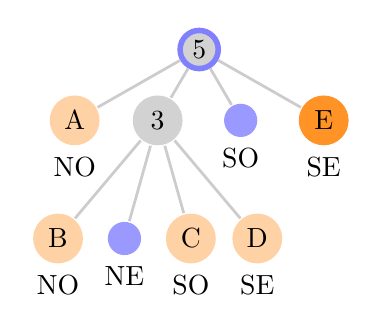
\begin{tikzpicture}[level 1/.style={sibling distance=5em, level distance=1.5cm},
                    level 2/.style={sibling distance=4em,level distance=2.5cm},
                    level distance = 1.5cm,
                    draw=gray!40,
                    fill=gray!40,
                    line width=1pt,
                    scale=0.6]
    \tikzstyle{internal}=[circle,fill=gray!35,minimum size=18pt,inner sep=2pt]
    \tikzstyle{external}=[internal, fill=orange!85];
    \tikzstyle{externaldisable}=[external, fill=orange!35];
    \tikzstyle{empty}=[internal, fill=blue!40, minimum size=12pt];
    \tikzstyle{actual}=[internal, draw=blue!50, minimum size=12pt,line width=2pt];


    \node[actual] {5}
        child { node[externaldisable,label=below:NO] {A}}
        child { node[internal] {3}
                child { node[externaldisable,label=below:NO] {B} }
                child { node[empty,label=below:NE] {} }
                child { node[externaldisable,label=below:SO] {C} }
                child { node[externaldisable,label=below:SE] {D} }
        }
        child { node[empty,label=below:SO] {} }
        child { node[external,label=below:SE] {E} };
\end{tikzpicture}
\end{center}

}

\frame
{
\frametitle{Barnes-Hut Tree Code}
\framesubtitle{Cálculo de la fuerza sobre un cuerpo}

Calcular la fuerza que ejerce \red{la red} sobre un \blue{cuerpo b},
comenzando con la raiz:

\begin{enumerate}
	\item<1-> \red{Si} el \green{nodo actual} es un \blue{nodo externo} (y no b).\\ Calcular y agregar fuerza.
	\item<2-> \red{Si no}, calcular $\frac{s}{d}$. Si $\frac{s}{d} < \theta$,
			nodo interno como un único cuerpo.\\Calcular y agregar fuerza.
	\item<3-> \red{Si no}, recursividad del procedimiento en cada \blue{hijo del nodo actual}.
\end{enumerate}
}

\frame
{
\frametitle{Barnes-Hut Tree Code}
\framesubtitle{Cálculo de la fuerza sobre un cuerpo}

\begin{itemize}
	\item Ejemplo, calcular la fuerza de la red sobre el \blue{cuerpo a}.
	\item Comenzaremos en la \red{raíz} (nodo interno).
	\begin{itemize}
		\item Representa CM de los 6 cuerpos.
		 \begin{itemize}
		 	\item a, b, c, d, e y f, con masas 1, 2, 3, 4, 5 y 6 Kg.
		 \end{itemize}
	\end{itemize}
\end{itemize}
El calculo de fuerza procede de la siguiente forma.
}

\frame
{
\frametitle{Barnes-Hut Tree Code}
\framesubtitle{Cálculo de la fuerza sobre un cuerpo}

\red{1.} El primer nodo examinado es la raíz.
\begin{itemize}
	\item Cociente entre A y CM. $\frac{s}{d} = \frac{100}{43.1} > \theta = 0.5$
	\item $\rightarrow$ Proceso recursivo dentro.
\end{itemize}

\begin{center}
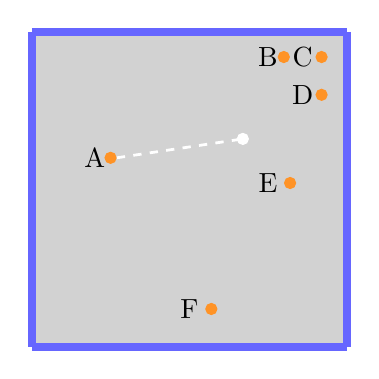
\begin{tikzpicture}[scale=0.4]
    \tikzstyle{square}=[rectangle,fill=gray!35, minimum size=4cm]
    \node[square] at (0,0) {};
    \filldraw[draw=orange!85, fill=orange!85] (-2.5,1)   circle (5pt)
                                              (3,4.2)    circle (5pt)
                                              (4.2,4.2)  circle (5pt)
                                              (4.2,3)    circle (5pt)
                                              (3.2,0.2)  circle (5pt)
                                              (0.7,-3.8) circle (5pt);

    \filldraw[draw=white!85, fill=white!85] (1.7,1.6) circle (5pt);

    \draw[draw=blue!60, line width=3pt] (-5,5) -- (5,5)
                                        (5,5)  -- (5,-5)
                                        (5,-5) -- (-5,-5)
                                        (-5,-5)-- (-5,5);

    \draw[draw=white!80, line width=1pt,dashed] (-2.3,1) -- (1.7,1.6);

    \draw (-3,1)    node {A}
          (2.5,4.2) node {B}
          (3.6,4.2) node {C}
          (3.6,3)   node {D}
          (2.5,0.2) node {E}
          (0,-3.8)  node {F};
\end{tikzpicture}
\hspace{0.5cm}
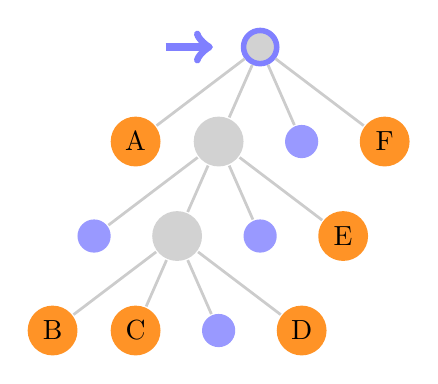
\begin{tikzpicture}[level 1/.style={sibling distance=5em, level distance=2cm},
                    level distance = 2cm,
                    draw=gray!40,
                    fill=gray!40,
                    line width=1pt,
                    scale=0.6,
                    ]
    \tikzstyle{internal}=[circle,fill=gray!35,minimum size=18pt,inner sep=2pt]
    \tikzstyle{external}=[internal, fill=orange!85];
    \tikzstyle{externaldisable}=[external, fill=orange!35];
    \tikzstyle{empty}=[internal, fill=blue!40, minimum size=12pt];
    \tikzstyle{actual}=[internal, draw=blue!50, minimum size=12pt,line width=2pt];


    \node[actual] (root) {}
            child { node[external] {A}}
            child { node[internal] {}
                child { node[empty] {} }
                child { node[internal] {}
                    child { node[external] {B}}
                    child { node[external] {C}}
                    child { node[empty] {}}
                    child { node[external] {D}}
                }
                child { node[empty] {} }
                child { node[external] {E} }
            }
            child { node[empty] {}}
            child { node[external] {F}}
        ;

    \path[draw,ultra thick,blue!50, line width=3pt,->] (-2,0) -- (-1,0);
\end{tikzpicture}

\end{center}

}

\frame
{
\frametitle{Barnes-Hut Tree Code}
\framesubtitle{Cálculo de la fuerza sobre un cuerpo}

\red{2.} El primer hijo es el cuerpo A
\begin{itemize}
	\item No ejerce fuerza sobre si mismo.
	\item $\rightarrow$ No hacemos nada.
\end{itemize}

\begin{center}
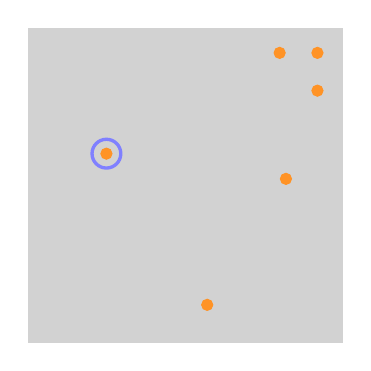
\begin{tikzpicture}[scale=0.4]
    \tikzstyle{square}=[rectangle,fill=gray!35, minimum size=4cm]
    \node[square] at (0,0) {};
    \filldraw[draw=orange!85, fill=orange!85] (-2.5,1) circle (5pt)
                                              (3,4.2)    circle (5pt)
                                              (4.2,4.2)  circle (5pt)
                                              (4.2,3)    circle (5pt)
                                              (3.2,0.2)  circle (5pt)
                                              (0.7,-3.8) circle (5pt);
    \draw[blue!50,line width=1.2pt] (-2.5,1) circle (13pt);

\end{tikzpicture}
\hspace{0.5cm}
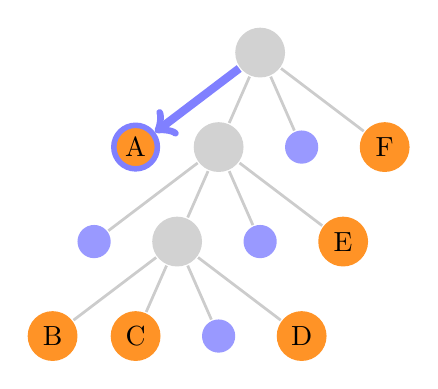
\begin{tikzpicture}[level 1/.style={sibling distance=5em, level distance=2cm},
                    level distance = 2cm,
                    draw=gray!40,
                    fill=gray!40,
                    line width=1pt,
                    scale=0.6,
                    radius=20,
                    ]
    \tikzstyle{internal}=[circle,fill=gray!35,minimum size=18pt,inner sep=2pt]
    \tikzstyle{external}=[internal, fill=orange!85];
    \tikzstyle{externaldisable}=[external, fill=orange!35];
    \tikzstyle{empty}=[internal, fill=blue!40, minimum size=12pt];
    \tikzstyle{actual}=[internal, draw=blue!50, minimum size=12pt,line width=2pt];
    \tikzstyle{actualN}=[external, draw=blue!50, minimum size=12pt,line width=2pt];


    \node[internal] (root) {}
            child { node[actualN](A) {A}}
            child { node[internal](in1) {}
                child { node[empty] {} }
                child { node[internal](in2) {}
                    child { node[external](B) {B}}
                    child { node[external](C) {C}}
                    child { node[empty] {}}
                    child { node[external](D) {D}}
                }
                child { node[empty] {} }
                child { node[external](E) {E} }
            }
            child { node[empty] {}}
            child { node[external](F) {F}}
        ;

    \path[draw,ultra thick,blue!50, line width=3pt,->] (root) -- (A);
\end{tikzpicture}

\end{center}
}


\frame
{
\frametitle{Barnes-Hut Tree Code}
\framesubtitle{Cálculo de la fuerza sobre un cuerpo}

\red{3.} Hijo representante NE (contiene b, c, d y e).
\begin{itemize}
	\item $\frac{s}{d} = \frac{50}{62.7} > \theta$.
	\item $\rightarrow$ Proceso recursivo dentro.
\end{itemize}
\begin{center}
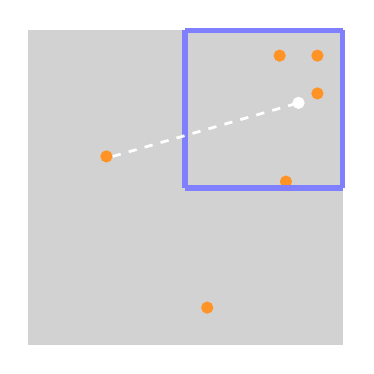
\begin{tikzpicture}[scale=0.4]
    \tikzstyle{square}=[rectangle,fill=gray!35, minimum size=4cm]
    \node[square] at (0,0) {};
    \filldraw[draw=orange!85, fill=orange!85] (-2.5,1) circle (5pt)
                                              (3,4.2)    circle (5pt)
                                              (4.2,4.2)  circle (5pt)
                                              (4.2,3)    circle (5pt)
                                              (3.2,0.2)  circle (5pt)
                                              (0.7,-3.8) circle (5pt);

    \filldraw[draw=white!85, fill=white!85] (3.6,2.7) circle (5pt);

    \draw[blue!50,line width=2pt] (0,0) -- (0,5)
                                  (0,5) -- (5,5)
                                  (5,5) -- (5,0)
                                  (5,0) -- (0,0);

    \draw[dashed,line width=1pt,white!85] (-2.3,1) -- (3.6,2.7);

\end{tikzpicture}
\hspace{0.5cm}
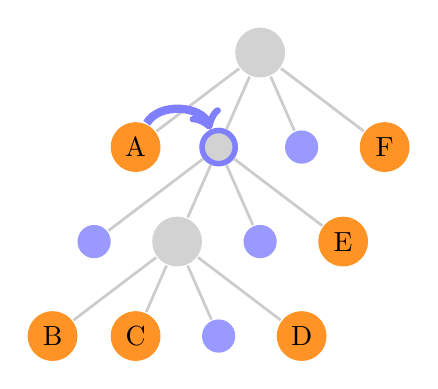
\begin{tikzpicture}[level 1/.style={sibling distance=5em, level distance=2cm},
                    level distance = 2cm,
                    draw=gray!40,
                    fill=gray!40,
                    line width=1pt,
                    scale=0.6,
                    radius=20,
                    ]
    \tikzstyle{internal}=[circle,fill=gray!35,minimum size=18pt,inner sep=2pt]
    \tikzstyle{external}=[internal, fill=orange!85];
    \tikzstyle{externaldisable}=[external, fill=orange!35];
    \tikzstyle{empty}=[internal, fill=blue!40, minimum size=12pt];
    \tikzstyle{actual}=[internal, draw=blue!50, minimum size=12pt,line width=2pt];
    \tikzstyle{actualN}=[external, draw=blue!50, minimum size=12pt,line width=2pt];


    \node[internal] (root) {}
            child { node[external](A) {A}}
            child { node[actual](in1) {}
                child { node[empty] {} }
                child { node[internal](in2) {}
                    child { node[external](B) {B}}
                    child { node[external](C) {C}}
                    child { node[empty] {}}
                    child { node[external](D) {D}}
                }
                child { node[empty] {} }
                child { node[external](E) {E} }
            }
            child { node[empty] {}}
            child { node[external](F) {F}}
        ;

    \path[draw,ultra thick,blue!50, line width=3pt,->] (A) edge[bend left=65] (in1);
\end{tikzpicture}

\end{center}

}

\frame
{
\frametitle{Barnes-Hut Tree Code}
\framesubtitle{Cálculo de la fuerza sobre un cuerpo}

\red{4.} Hijo representante NE del padre (contiene b, c y d).
\begin{itemize}
	\item $\frac{s}{d} = 25/66.9 < \theta$.
	\item $\rightarrow$ Se calcula la fuerza como un sólo nodo.
\end{itemize}

\begin{center}
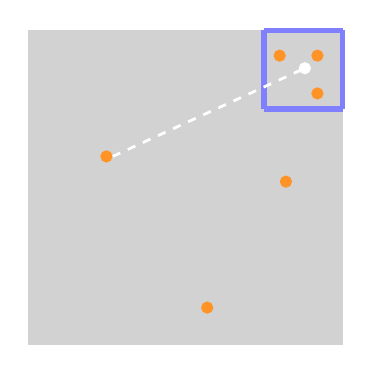
\begin{tikzpicture}[scale=0.4]
    \tikzstyle{square}=[rectangle,fill=gray!35, minimum size=4cm]
    \node[square] at (0,0) {};
    \filldraw[draw=orange!85, fill=orange!85] (-2.5,1) circle (5pt)
                                              (3,4.2)    circle (5pt)
                                              (4.2,4.2)  circle (5pt)
                                              (4.2,3)    circle (5pt)
                                              (3.2,0.2)  circle (5pt)
                                              (0.7,-3.8) circle (5pt);

    \filldraw[draw=white!85, fill=white!85] (3.8,3.8) circle (5pt);

    \draw[blue!50,line width=2pt] (2.5,2.5) -- (2.5,5)
                                  (2.5,5) -- (5,5)
                                  (5,5) -- (5,2.5)
                                  (5,2.5) -- (2.5,2.5);

    \draw[dashed,line width=1pt,white!85] (-2.3,1) -- (3.8,3.8);

\end{tikzpicture}
\hspace{0.5cm}
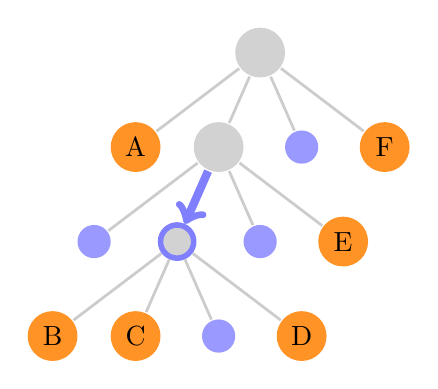
\begin{tikzpicture}[level 1/.style={sibling distance=5em, level distance=2cm},
                    level distance = 2cm,
                    draw=gray!40,
                    fill=gray!40,
                    line width=1pt,
                    scale=0.6,
                    radius=20,
                    ]
    \tikzstyle{internal}=[circle,fill=gray!35,minimum size=18pt,inner sep=2pt]
    \tikzstyle{external}=[internal, fill=orange!85];
    \tikzstyle{externaldisable}=[external, fill=orange!35];
    \tikzstyle{empty}=[internal, fill=blue!40, minimum size=12pt];
    \tikzstyle{actual}=[internal, draw=blue!50, minimum size=12pt,line width=2pt];
    \tikzstyle{actualN}=[external, draw=blue!50, minimum size=12pt,line width=2pt];


    \node[internal] (root) {}
            child { node[external](A) {A}}
            child { node[internal](in1) {}
                child { node[empty] {} }
                child { node[actual](in2) {}
                    child { node[external](B) {B}}
                    child { node[external](C) {C}}
                    child { node[empty] {}}
                    child { node[external](D) {D}}
                }
                child { node[empty] {} }
                child { node[external](E) {E} }
            }
            child { node[empty] {}}
            child { node[external](F) {F}}
        ;

    \path[draw,ultra thick,blue!50, line width=3pt, ->] (in1) -- (in2);
\end{tikzpicture}

\end{center}

}

\frame
{
\frametitle{Barnes-Hut Tree Code}
\framesubtitle{Cálculo de la fuerza sobre un cuerpo}

\red{5.} El siguiente hijo es el que contiene el cuerpo e.
\begin{itemize}
	\item  Este es un nodo externo.
	\item $\rightarrow$ Calculamos fuerza entre a y e.
\end{itemize}

\begin{center}
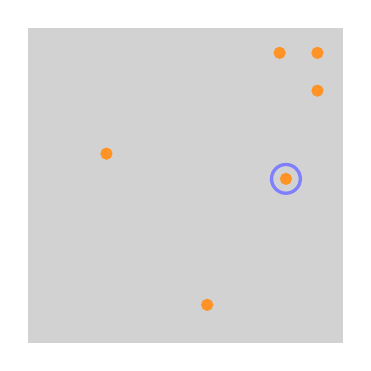
\begin{tikzpicture}[scale=0.4]
    \tikzstyle{square}=[rectangle,fill=gray!35, minimum size=4cm]
    \node[square] at (0,0) {};
    \filldraw[draw=orange!85, fill=orange!85] (-2.5,1) circle (5pt)
                                              (3,4.2)    circle (5pt)
                                              (4.2,4.2)  circle (5pt)
                                              (4.2,3)    circle (5pt)
                                              (3.2,0.2)  circle (5pt)
                                              (0.7,-3.8) circle (5pt);

    \draw[blue!50,line width=1.2pt] (3.2,0.2) circle (13pt);

\end{tikzpicture}
\hspace{0.5cm}
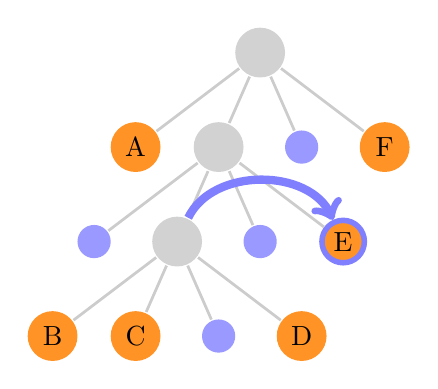
\begin{tikzpicture}[level 1/.style={sibling distance=5em, level distance=2cm},
                    level distance = 2cm,
                    draw=gray!40,
                    fill=gray!40,
                    line width=1pt,
                    scale=0.6,
                    radius=20,
                    ]
    \tikzstyle{internal}=[circle,fill=gray!35,minimum size=18pt,inner sep=2pt]
    \tikzstyle{external}=[internal, fill=orange!85];
    \tikzstyle{externaldisable}=[external, fill=orange!35];
    \tikzstyle{empty}=[internal, fill=blue!40, minimum size=12pt];
    \tikzstyle{actual}=[internal, draw=blue!50, minimum size=12pt,line width=2pt];
    \tikzstyle{actualN}=[external, draw=blue!50, minimum size=12pt,line width=2pt];


    \node[internal] (root) {}
            child { node[external](A) {A}}
            child { node[internal](in1) {}
                child { node[empty] {} }
                child { node[internal](in2) {}
                    child { node[external](B) {B}}
                    child { node[external](C) {C}}
                    child { node[empty] {}}
                    child { node[external](D) {D}}
                }
                child { node[empty] {} }
                child { node[actualN](E) {E} }
            }
            child { node[empty] {}}
            child { node[external](F) {F}}
        ;

    \path[draw,ultra thick,blue!50, line width=3pt, ->] (in2) edge [bend left=65] (E);
\end{tikzpicture}

\end{center}

}

\frame
{
\frametitle{Barnes-Hut Tree Code}
\framesubtitle{Cálculo de la fuerza sobre un cuerpo}

\red{6.} Volvemos al nivel anterior, para ver otro hijo.
\begin{itemize}
	\item Este es un nodo externo.
	\item $\rightarrow$ Calculamos fuerza entre a y f. 
\end{itemize}

\begin{center}
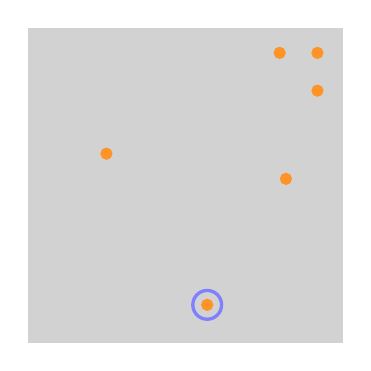
\begin{tikzpicture}[scale=0.4]
    \tikzstyle{square}=[rectangle,fill=gray!35, minimum size=4cm]
    \node[square] at (0,0) {};
    \filldraw[draw=orange!85, fill=orange!85] (-2.5,1) circle (5pt)
                                              (3,4.2)    circle (5pt)
                                              (4.2,4.2)  circle (5pt)
                                              (4.2,3)    circle (5pt)
                                              (3.2,0.2)  circle (5pt)
                                              (0.7,-3.8) circle (5pt);

    \draw[blue!50,line width=1.2pt] (0.7,-3.8) circle (13pt);

\end{tikzpicture}
\hspace{0.5cm}
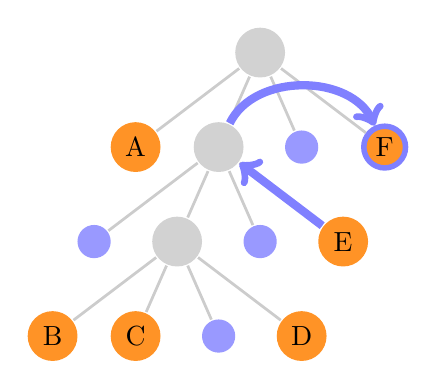
\begin{tikzpicture}[level 1/.style={sibling distance=5em, level distance=2cm},
                    level distance = 2cm,
                    draw=gray!40,
                    fill=gray!40,
                    line width=1pt,
                    scale=0.6,
                    radius=20,
                    ]
    \tikzstyle{internal}=[circle,fill=gray!35,minimum size=18pt,inner sep=2pt]
    \tikzstyle{external}=[internal, fill=orange!85];
    \tikzstyle{externaldisable}=[external, fill=orange!35];
    \tikzstyle{empty}=[internal, fill=blue!40, minimum size=12pt];
    \tikzstyle{actual}=[internal, draw=blue!50, minimum size=12pt,line width=2pt];
    \tikzstyle{actualN}=[external, draw=blue!50, minimum size=12pt,line width=2pt];


    \node[internal] (root) {}
            child { node[external](A) {A}}
            child { node[internal](in1) {}
                child { node[empty] {} }
                child { node[internal](in2) {}
                    child { node[external](B) {B}}
                    child { node[external](C) {C}}
                    child { node[empty] {}}
                    child { node[external](D) {D}}
                }
                child { node[empty] {} }
                child { node[external](E) {E} }
            }
            child { node[empty] {}}
            child { node[actualN](F) {F}}
        ;

    \path[draw,ultra thick,blue!50, line width=3pt, ->] (E) -- (in1);
    \path[draw,ultra thick,blue!50, line width=3pt, ->] (in1) edge [bend left=65] (F);
\end{tikzpicture}

\end{center}

}

\frame
{
\frametitle{Barnes-Hut Tree Code}
\framesubtitle{Cálculo de la fuerza sobre un cuerpo}
\red{7.} Finalmente, en cada paso vamos sumando las fuerzas calculadas,
para obtener la fuerza total de la red sobre el \blue{cuerpo a}.
}
